\section{\acrlong{lda}}\label{sec:lda}
\Gls{lda} is topic model method. The objective of topic modeling is to infer topics (collections of words) in a document set.

\begin{definition}\label{def:topic}
	\textit{A topic is a distribution over words in a corpus}
\end{definition}

The result consists of a topic-word distribution matrix $\beta$, which for each topic gives a distribution of words belonging to said topic, and a document-topic distribution matrix $\theta$ which for each document gives a distribution of topics to which the document belongs to.

\citeauthor{lda} \cite{lda} introduce \gls{lda}, which has since become a staple within topic modeling.
\gls{lda} works under the assumption that documents are generated from a specific generative process, and tries to reverse engineer this process.
This generative process assumes that documents are random mixtures of latent topics and that each topic is a distribution over all the words in the corpus.

This process generates $K$ topics and $D$ documents containing $N_{d}$ words, where $d$ is a document in $D$.
The generative process has two Dirichlet distributions $Dir(\alpha)$ for the document-topic relation and $Dir(\eta)$ for the topic-word relation.

\begin{figure}[h]
	\centering
	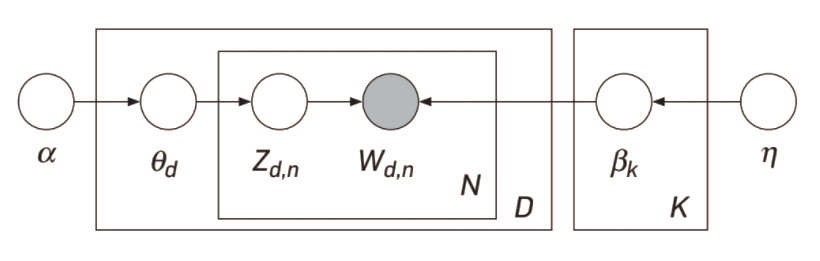
\includegraphics[width=0.5\textwidth]{figures/Smoothed_LDA.jpg}
	\caption{Plate notation for \gls{lda}. Boxes symbolize repeated processes, shaded elements are observed information. Image is from \url{https://en.wikipedia.org/wiki/Latent_Dirichlet_allocation}}
	\label{fig:lda}
\end{figure}
\vejleder[inline]{beskriv inference og learning af modelen i appendix}
From these Dirichlet distributions, we can sample two multinomial distributions: document-topic $\theta$ and topic-word $\beta$.
These Dirichlet distributions are tuned with the hyperparameters $\alpha$ and $\eta$, which adjust the entropy of the sampled distributions.
An $\alpha$ value near 1 causes each document to be distributed over almost all topics, while an $\alpha$ value near 0 causes each document to be distributed over only a few topics.
Similarly $\eta$ will adjust how many words each topic contains.
This also has the added consequence that a high $\alpha$ will make documents appear more similar, and a high $\eta$ will make topics appear more similar.

Using $\theta$ and $\beta$, we can sample concrete topics $Z$ from documents, and concrete words $W$ from topics.
\autoref{fig:lda} gives an overview of the assumed generative process.

\todo[inline]{mention the limitations of lda.}